\documentclass[8pt]{article}
 
\usepackage[margin=.8in]{geometry} 
\usepackage{amsmath,amsthm,amssymb}
\usepackage{marvosym,enumerate,color,mathrsfs,graphicx,epstopdf}
\usepackage{enumitem}
%\setenumerate{listparindent=\parindent}
\def\cc{\color{blue}}
%\usepackage[dvipsnames]{xcolor}
\usepackage[normalem]{ulem}
\usepackage{bm}
\usepackage{mathtools}
\usepackage{mathrsfs}
\usepackage{verbatim}
\usepackage{tikz}
\usepackage[utf8]{inputenc}
\usepackage{hyperref}
\usepackage{courier}
\usepackage{fullpage}
\usepackage{graphicx}
\usepackage{float}
\hypersetup{
	%colorlinks,
	%citecolor=black,
	%filecolor=black,
	%linkcolor=blue,
	%urlcolor=black
}


%\usepackage{multirow}

%Line Numbering
\usepackage[mathlines]{lineno}
%\linenumbers
 
\newcommand{\N}{\mathbb{N}}
\newcommand{\Z}{\mathbb{Z}}
\newcommand{\R}{\mathbb{R}}
\newcommand{\C}{\mathbb{C}}
\newcommand{\Q}{\mathbb{Q}}
%\newcommand{\dell}{\partial}
\newcommand{\abs}[1]{\left\lvert{#1}\right\rvert}
\newcommand{\dx}{\mathrm{d}x}
\newcommand{\M}{\mathscr{M}}
\newcommand{\E}{\mathscr{E}}
\newcommand{\B}{\mathscr{B}}
\newcommand{\scr}[1]{\mathscr{#1}}
\newcommand{\Ns}{\mathscr{N}}
\newcommand{\nm}{\mathrel{\unlhd}}
\newcommand{\stcomp}[1]{{#1}^{\mathsf{c}}}
\newcommand{\closure}[1]{\overline{#1}}
\newcommand{\diam}{\operatorname{diam}}
\newcommand{\dist}{\operatorname{dist}}
\newcommand{\sgn}{\operatorname{sgn}}
\newcommand{\norm}[1]{\left\lVert{#1}\right\rVert}
\newcommand{\LR}[1]{\left\langle{#1}\right\rangle}

\theoremstyle{definition}
\newtheorem{theorem}{Theorem}
\newtheorem*{theorem*}{Theorem}
\newtheorem{lemma}[theorem]{Lemma}
\newtheorem{proposition}[theorem]{Proposition}
\newtheorem*{proposition*}{Proposition}
\newtheorem{definition}[theorem]{Definition}
\newtheorem*{definition*}{Definition}
\newtheorem{remark}[theorem]{Remark(s)}
\newtheorem*{remark*}{Remark(s)}
\newtheorem{corollary}[theorem]{Corollary}
\newtheorem*{corollary*}{Corollary}
\newtheorem{innerexercise}{Exercise}
\newenvironment{exercise}[1]
  {\renewcommand\theinnerexercise{#1}\innerexercise}
  {\endinnerexercise}

% Upper and lower integrals
%\def\upint{\mathchoice%
%    {\mkern13mu\overline{\vphantom{\intop}\mkern7mu}\mkern-20mu}%
%    {\mkern7mu\overline{\vphantom{\intop}\mkern7mu}\mkern-14mu}%
%    {\mkern7mu\overline{\vphantom{\intop}\mkern7mu}\mkern-14mu}%
%    {\mkern7mu\overline{\vphantom{\intop}\mkern7mu}\mkern-14mu}%
%  \int}
%\def\lowint{\mkern3mu\underline{\vphantom{\intop}\mkern7mu}\mkern-10mu\int}

\title{Numerical Analysis -- Homework 3}
\author{James Diffenderfer}
\date{\today}

%%%%%%%%%%%%%%%%%%%%%%%%%%%%%%%%%%%%%%
\begin{document}

\maketitle
%\tableofcontents

%\newpage

\begin{exercise}{1}
For $a = x_0 < x_1 < \ldots < x_n = b$ and a function $f \in C[a,b]$, show that the interpolation problem has a unique solution 
\begin{align}
Q(x) = \sum_{j = 0}^{n} c_j e^{j x}
\end{align}
with $Q(x_i) = f(x_i)$ for all $i$. \emph{Hint}: Reduce to a usual polynomial interpolation problem.
\end{exercise}

\begin{proof}
Define $g : (0, \infty) \to \mathbb{R}$ by $g (z) = (f \circ \ln) (z)$. Since $f \in C [a, b]$ and $\ln \in C(0, \infty)$ we have that $g \in C [e^a, e^b]$. Now perform a change of variables by defining $z = e^x$. Since $e^x$ is a strictly increasing function on $\mathbb{R}$ and $a = x_0 < \ldots < x_n = b$, by defining $z_i = e^{x_i}$, for $0 \leq i \leq n$, we have that $e^a = z_0 < z_1 < \ldots < z_n = e^b$.  Since $g \in C [e^a, e^b]$ and $e^a = z_0 < z_1 < \ldots < z_n = e^b$, by Theorem 3.2 (in \emph{Numerical Analysis} by Burden and Faires) $$P(z) = \sum_{j = 0}^{n} g(z_j) L_{n, j} (z),$$ is the unique polynomial of degree at most $n$ satisfying $g(z_j) = P(z_j)$ for $0 \leq j \leq n$. Here the functions are $L_{n, j} (z) = \prod_{k \neq j} \frac{(z - z_k)}{(z_j - z_k)}, 0 \leq j \leq n$. So by defining $$E_{n, j} (x) = \prod_{k \neq j} \frac{e^x - e^{x_k}}{e^{x_j} - e^{x_k}}$$ we now have that $E_{n, j} (x_i) = L_{n, j} (z_i) = \delta_{ij}$. Hence, letting $$Q(x) = \sum_{j = 0}^{n} f(x_j) E_{n, j} (x)$$ it follows that 
\begin{align}
Q(x) = \sum_{j = 0}^{n} f(x_j) E_{n, j} (x) = \sum_{j = 0}^{n} f(\ln (e^{x_j})) L_{n, j} (z) = \sum_{j = 0}^{n} g (z_j) L_{n, j} (z)= P(z),
\end{align}
namely, $Q(x_i) = f(x_i)$, for $0 \leq i \leq n$. We prove uniqueness by way of contradiction. Accordingly, suppose that there exist $Q (x)$ and $R(x)$ satisfying (1) with $Q(x) \neq R(x)$. By our proof of existence, there exist corresponding polynomials $P(z)$ and $M(z)$ satisfying the equality in (2) for $Q(x)$ and $R(x)$, respectively. Thus, by the uniqueness of the interpolating polynomial from Theorem 3.2 we have that $Q(x) = P(z) = M(z) = R(x)$, a contradiction to $Q(x) \neq R(x)$. Thus, $Q(x)$ is unique.
%Since $\ln : \mathbb{R} \to \mathbb{R}$ is a bijective function and $x = \ln z$, the uniqueness of $Q(x)$ follows immediately from the uniqueness of $P(z)$.
\end{proof}

%Under this change of variables, observe that the condition $f(x_i) = Q(x_i)$ is equivalent to $$f(x_i) = \sum_{j = 0}^{n} c_j e^{j x_i} = \sum_{j = 0}^{n} c_j z_{i}^{j}.$$ Hence, by defining $g(z) = \sum_{j = 0}^{n} c_j z^j$ and $z_i = e^{x_i}$, for $0 \leq i \leq n$, the above condition is equivalent to $f(x_i) = g(z_i)$, for $0 \leq i \leq n$.
\newpage

\begin{exercise}{2}
Consider the inner product on $C[1, 2]$, $$\langle f, g \rangle = \int_{1}^{2} f(x) g(x) e^{-x} dx.$$
\begin{enumerate}
	\item[(a)] Starting with the basis $\{1, x, x^2 \}$ for $\mathcal{P}_2 [1, 2]$ use Gram-Schmidt to determine the first three orthonormal polynomials on $[1, 2]$ with respect to the inner product.
	\item[(b)] Find the order 2 best least squares approximation for $f(x) = e^{x}$ on $[1, 2]$ with respect to the given inner product.
\end{enumerate}
\end{exercise}

\begin{proof}[Proof of (a)]
Using Gram-Schmidt, the first orthonormal polynomial on $[1, 2]$ with respect to the given inner product is $$q_0 (x) = \frac{e}{\sqrt{e - 1}} \approx 2.073706473.$$ Then $\displaystyle q_1 (x) = \frac{p_1 (x)}{\langle p_1 (x), p_1 (x) \rangle^{1/2}}$, where $p_1 (x) = x - \langle x, q_0 (x) \rangle q_0 (x)$. Since
\begin{align*}
\langle x, q_0 (x) \rangle &= \frac{e}{\sqrt{e - 1}} \int_{1}^{2} x e^{-x} dx \\
&= \frac{e}{\sqrt{e - 1}} \left( \left[ -x e^{-x} \right]_{1}^{2} - \int_{1}^{2} - e^{-x} dx \right) \\
&= \frac{e}{\sqrt{e - 1}} \left( -2 e^{-2} + e^{-1} - e^{-2} + e^{-1} \right) \\
&= \frac{e}{\sqrt{e - 1}} \left( -3 e^{-2} + 2 e^{-1} \right) \\
&\approx 0.683810998,
\end{align*}
we have that $p_1 (x) = x - 1.418023293$. Hence, letting $k = 1.418023293$, we have
\begin{align*}
\langle p_1 (x), p_1 (x) \rangle &= \int_{1}^{2} \left( x^2 - 2 k x + k^2 \right) e^{-x} dx \\
&= \int_{1}^{2} x^2 e^{-x} dx - 2 k \int_{1}^{2} x e^{-x} dx + k^2 \int_{1}^{2} e^{-x} dx \\
&= \left[ -x^2 e^{-x} - 2 x e^{-x} - 2 e^{-x} \right]_{1}^{2} - 2k [-3 e^{-2} + 2 e^{-1}] + k^2 \left[ -e^{-x} \right]_{1}^{2} \\
&= -10 e^{-2} + 5 e^{-1} - 2 k [-3 e^{-2} + 2 e^{-1}] + k^2 [e^{-1} - e^{-2}] \\
%&= -10 e^{-2} + 5 e^{-1} - 8 e^{-2} + 28 e^{-3} - 34 e^{-4} + 21 e^{-5} - 9 e^{-6} \\
%&= 5 e^{-1} - 18 e^{-2} + 28 e^{-3} - 34 e^{-4} + 21 e^{-5} - 9 e^{-6} \approx 0.293856417.
&\approx 0.018446892.
\end{align*}
Thus, $$q_1 (x) = \frac{x - 1.418023293}{\sqrt{0.018446892}} = 7.362721909 x - 10.44051117.$$ Next, $\displaystyle q_2 (x) = \frac{p_2 (x)}{\langle p_2 (x), p_2 (x) \rangle^{1/2}}$, where $p_2 (x) = x^2 - \langle x^2, q_1 (x) \rangle q_1 (x) - \langle x^2, q_0 (x) \rangle q_0 (x)$. Using a computer we find that 
\begin{align*}
\langle x^2, q_0 (x) \rangle \approx 1.0079133634 \ \ \text{and} \ \ \langle x^2, q_1 (x) \rangle \approx 0.3983825436.
\end{align*}
Hence, 
\begin{align*}
\langle x^2, q_0 (x) \rangle q_0 (x) \approx 2.09011647 \ \ \text{and} \ \ \langle x^2, q_1 (x) \rangle q_1 (x) \approx 2.93317988197 x - 4.15931739645.
\end{align*}
Thus, $p_{2} (x) = x^2 - 2.93317988197 x + 2.06920092645.$ Since $$\langle p_2 (x), p_2 (x) \rangle \approx 0.001238094453$$ we conclude that $$q_2 (x) = \frac{x^2 - 2.93317988197 x + 2.06920092645}{0.03518656637} = 28.419937 x^2 - 83.360787 x + 58.80656.$$
\end{proof}

\begin{proof}[Proof of (b)]
Define $P : C [1, 2] \to \mathcal{P}_2 [1, 2]$ by $$P f = \sum_{j = 0}^{2} \langle f, q_j (x) \rangle q_j (x),$$ for all $f \in C [1, 2]$. By our theorem we have that $w = P e^{x}$ minimizes the value $\| w - e^{x} \|$ over all $w \in \mathcal{P}_2 [1, 2]$. Since 
\begin{align*}
\langle e^x, q_0 (x) \rangle = 2.073706473, \ \ \langle e^x, q_1 (x) \rangle = 0.6035716935, \ \ \text{and} \ \ \langle e^x, q_2 (x) \rangle = 0.078565833
\end{align*}
we have that 
\begin{align*}
P e^{x} &= 0.078565833 \ q_2 (x) + 0.6035716935 \ q_1 (x) + 2.073706473 \ q_0 (x) \\
&= (2.23284 x^2 - 6.54931 x + 4.62019) + (4.44393 x - 6.3016) + 4.30025853 \\
&= 2.23284 x^2 - 2.10538 x + 2.61885.
\end{align*}
For a comparison of this polynomial to $e^x$, consider the plot of both functions in Figure 1.
\end{proof}
\begin{figure}[H]
	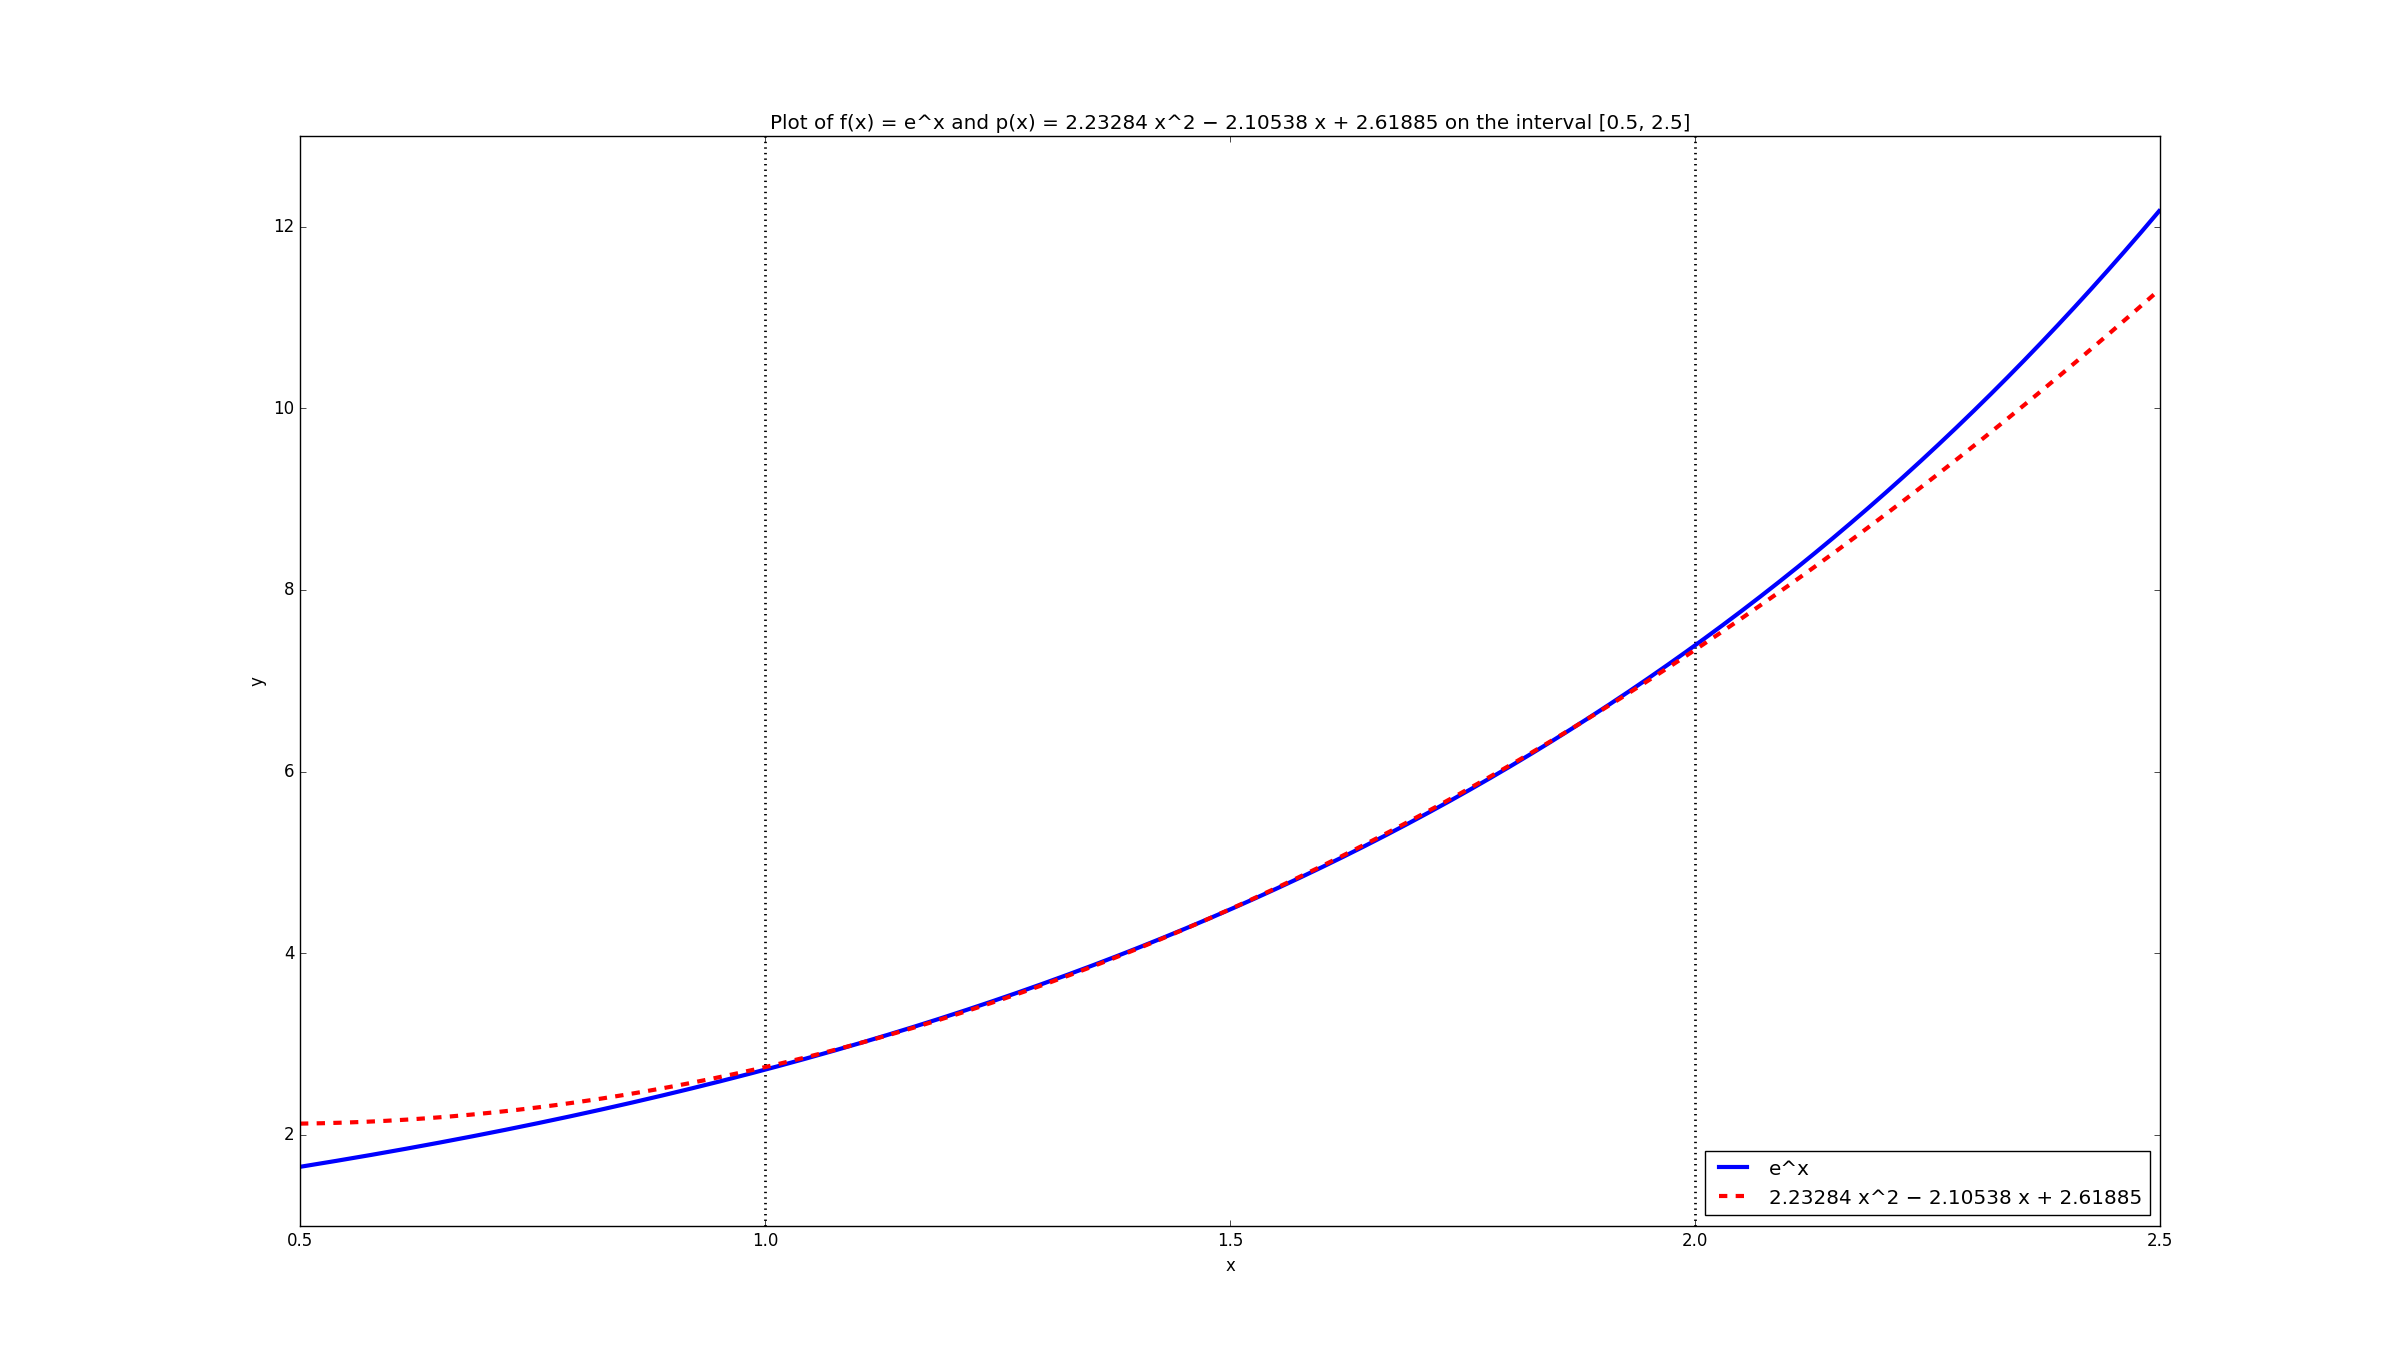
\includegraphics[trim={6cm, 0, 5cm, 2cm}, clip, width=\textwidth]{ortho_plot.png}
	\vspace{-10mm}
	\caption{Plot of $f(x) = e^x$ (solid line) and $p(x) = 2.23284 x^2 - 2.10538 x + 2.61885$ (dashed line), the polynomial constructed in 2 (a).}
	\label{Figure 1}
\end{figure}


\begin{exercise}{3}
Let $f(x) = \frac{1}{1 + x^2}$ on $[-5, 5]$.
\begin{enumerate}
	\item[(a)] Write a program which uses Newton divided differences to find the interpolating polynomial $p$ to $f$ with respect to $n = 10$ uniformly spaced nodes.
	\item[(b)] Evaluate $p(.4835)$ and compute the absolute error $| p(.4835) - f(.4835)|$.
\end{enumerate}
\end{exercise}

\begin{proof}[Code, experiments, and results]
The code is included on the final page of the homework. The program was coded using C++ and Figure 2 was generated using the 'matplotlib' package in python. Instead of computing the coefficients of the interpolating polynomial I used a recursion to compute values in my program. The output from the program I wrote is listed below: $$\texttt{p(0.4835) = 0.852867} \ \ \ \text{and} \ \ \ \texttt{|p(0.4835) - f(0.4835)| = 0.0423448}.$$

\begin{figure}[H]
	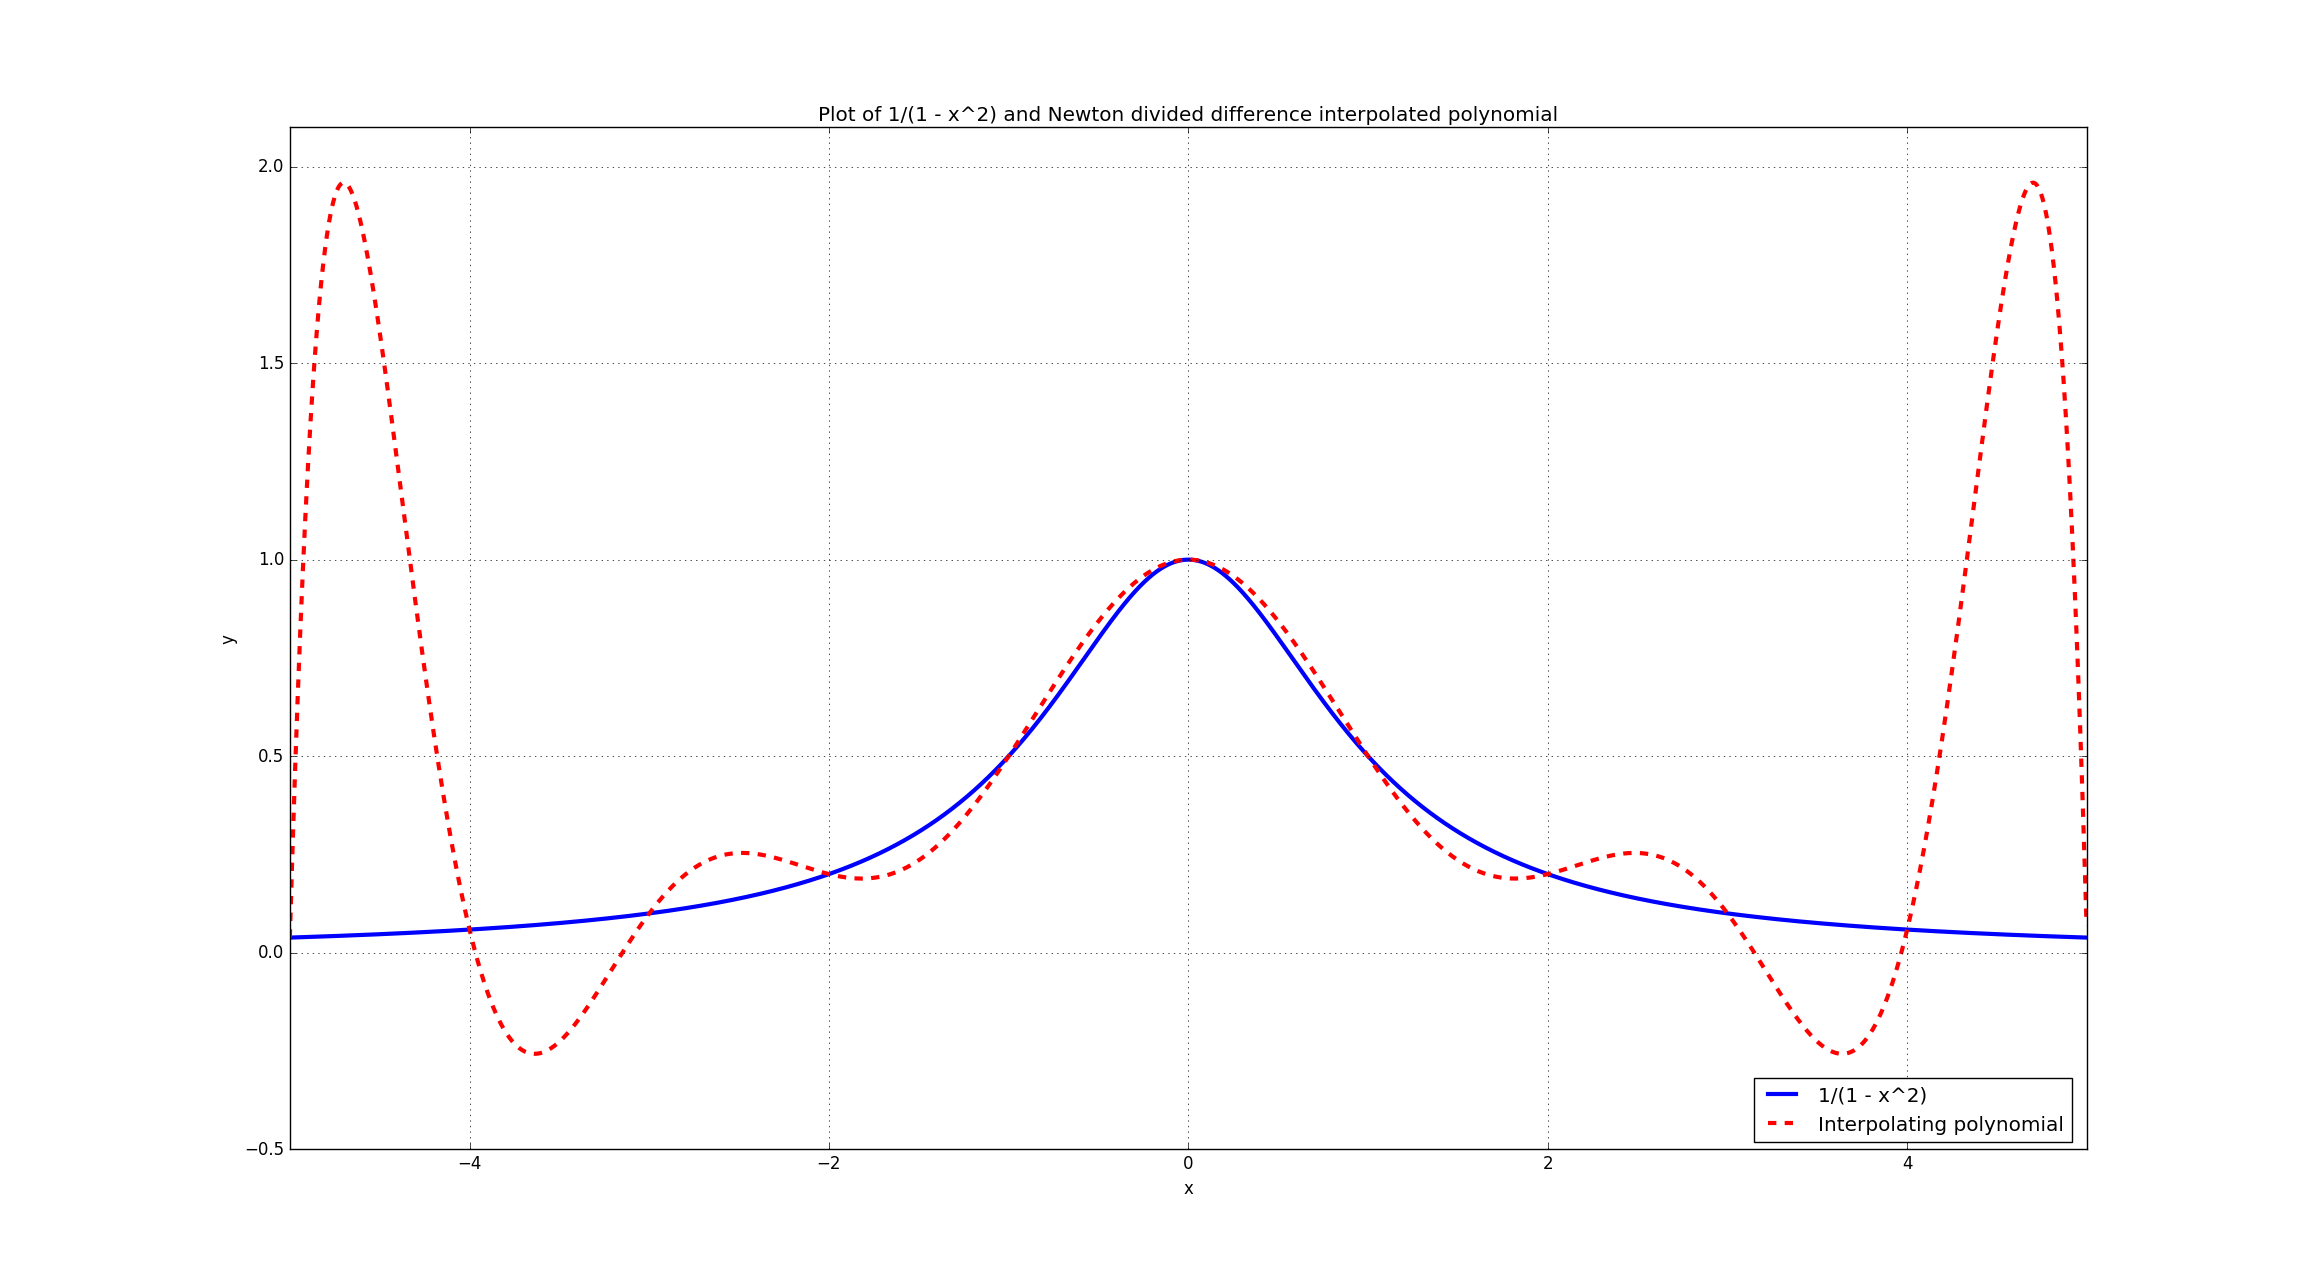
\includegraphics[trim={6cm, 0, 5cm, 2cm}, clip, width=\textwidth]{newtondd11.png}
	\vspace{-10mm}
	\caption{Plot of $f(x) = \frac{1}{1 + x^2}$ (solid line) and $p(x)$, the interpolated polynomial generated by Newton divided differences (dashed line).}
	\label{Figure 2}
\end{figure}
\end{proof}


\begin{exercise}{4}
If $f \in C^{2n + 2} [a, b]$ and $x_0, \ldots, x_n$ are distinct points in $[a, b]$ and $H_{2n + 1}$ is the corresponding Hermite polynomial, show that for $t \in [a, b]$ $$f(t) = H_{2n + 1} (t) + \frac{(t - x_0)^2 \cdots (t - x_n)^2}{(2n + 2)!} f^{(2n + 2)} (\eta),$$ for some $\eta \in [a, b]$.
\end{exercise}

\begin{proof}
Begin by defining $E(x) = f(x) - H_{2n + 1} (x)$, $w(x) = (x - x_0)^2 \cdots (x - x_n)^2$, and $$G(x) = E(x) - \frac{w (x)}{w (t)} E(t).$$ Based on these choices, we observe that 
\begin{enumerate}
	\item [(i)] $E (x_i) = f(x_i) - H_{2n + 1} (x_i) = 0$, for $0 \leq i \leq n$.
	\item [(ii)] $G(x_i) = E(x_i) - \frac{w (x_i)}{w (t)} E(t) = 0 - 0 = 0$, for $0 \leq i \leq n$.
	\item [(iii)] $G(t) = E(t) - \frac{w (t)}{w (t)} E(t) = 0$.
\end{enumerate}
By definition $G \in C^{(2n + 2)} [a, b]$. From (ii) and (iii) $G$ has $n + 2$ distinct zeros in $[a, b]$. By Rolle's Theorem, there exist $\xi_i \in (a, b)$, for $0 \leq i \leq n$, such that 
\begin{enumerate}
	\item [(a)] $G'(\xi_i) = 0$, for $0 \leq i \leq n$
	\item [(b)] $\xi_i \neq x_j$, for $0 \leq i, j \leq n$
	\item [(c)] $\xi_i \neq t$, for $0 \leq i \leq n$.
\end{enumerate}
Since $G'(x_i) = E'(x_i) - \frac{w'(x_i)}{w(t)^2} E(t) = 0$, for $0 \leq i \leq n$, $G'(x)$ has $2n + 2$ distinct roots in $(a, b)$, namely $\{x_0, x_1, \ldots, x_n, \xi_0, \xi_1, \ldots, \xi_n \}$. Thus, Generalized Rolle's Theorem yields that there exists a $\eta \in (a,b)$ with $G^{(2n + 2)} (\eta) = 0$. Computing derivatives with respect to $x$ we find that $$w^{(2n + 2)} (x) = (2n + 2)! \ \ \ \text{and} \ \ \ E^{(2n + 2)} (x) = f^{(2n + 2)} (x),$$ where the second equality holds since $H_{2n + 1}^{(2n + 2)} (x) = 0$. Hence,
\begin{align*}
G^{(2n + 2)} (x) &= f^{(2n + 2)} (x) - \frac{w^{(2n + 2)} (x)}{w(t)} E(t) \\
&= f^{(2n + 2)} (x) - \frac{(2n + 2)!}{w(t)} E(t).
\end{align*}
Substituting $x = \eta$ we get that $$E(t) = \frac{f^{(2n + 2)} (\eta)}{(2n + 2)!} w(t),$$ the desired result.
\end{proof}


\begin{exercise}{5}
Fix $n$. For the basic Lagrange polynomials $$L_k (x) = \prod_{i \neq j} \frac{x - x_j}{x_i - x_j},$$ for $k = 0, \ldots, n$. Show that $$\sum_{j = 0}^{n} L_{j} (x) = 1,$$ for all $x$.
\end{exercise}

\begin{proof}
Define the degree $n$ polynomial $p(x) = 1 - \sum_{j = 0}^{n} L_j (x)$. Since $L_j (x_i) = \delta_{ij}$ we have that $$p(x_j) = 1 - L_j (x_j) = 1 - 1 = 0,$$ for $0 \leq j \leq n$. Hence, $p(x)$ has $n + 1$ distinct roots. However, since $\deg p \leq n$ it follows that $p(x) \equiv 0$. Thus, we conclude that $\sum_{j = 0}^{n} L_j (x) = 1$. 
\end{proof}

\end{document}

%Failed attempt at problem 2
Letting $$c = \sqrt{5 e^{-1} - 2 e^{-2} - 20 e^{-3} + 2 e^{-4} + 21 e^{-5} - 9 e^{-6}} \approx 0.542085248$$ we have that 
\begin{align*}
\langle x^2, q_0 (x) \rangle = \int_{1}^{2} x^2 e^{-x} dx = -10 e^{-2} + 5 e^{-1}
\end{align*}
and
\begin{align*}
\langle x^2, q_1 (x) \rangle &= \frac{1}{c^2} \int_{1}^{2} (x + 3 - 2 e)^2 e^{-x} dx \\
&= \frac{1}{c^2} \left[ \int_{1}^{2} x^2 e^{-x} dx + 2 (3 - 2 e) \int_{1}^{2} x e^{-x} dx + (3 - 2 e)^2 \int_{1}^{2} e^{-x} dx \right] \\
&= \frac{1}{c^2} \left[ -10 e^{-2} + 5 e^{-1} + 2 (3 - 2 e) k + (3 - 2 e)^2 (e^{-1} - e^{-2}) \right] \\
&= \frac{1}{c^2} \left( 4e - 8 + 2 e^{-1} - e^{-2} \right).
\end{align*}
Hence, $$\langle x^2, q_0 (x) \rangle q_0 (x) = -10 e^{-2} + 5 e^{-1}$$ and 
\begin{align*}
\langle x^2, q_1 (x) \rangle q_1 (x) &= \frac{1}{c^2} \left( 4e - 8 + 2 e^{-1} - e^{-2} \right) \frac{x + 3 - 2 e}{c} \\
&= \frac{(x + 3 - 2e)(4 e - 8 + 2 e^{-1} - e^{-2})}{c^3} \\
&= \frac{(x + 3 - 2e)(4 e^{3} - 8 e^{2} + 2 e - 1)}{e^{2} c^3} \\
&= \frac{(x + 3 - 2e)(4 e^{3} - 8 e^{2} + 2 e - 1)}{e^{2} (5 e^{3} - 2 e^{2} + 2 e + 2 + 21 e^{-1} - 9 e^{-2})^{3/2}} \\
&= \frac{(x + 3 - 2e)(4 e^{3} - 8 e^{2} + 2 e - 1)}{(5 e^{5} - 2 e^{4} + 2 e^{3} + 2 e^{2} + 21 e - 9) \sqrt{5 e^{3} - 2 e^{2} + 2 e + 2 + 21 e^{-1} - 9 e^{-2}}}
\end{align*}
Thus, $$p_{3} (x) = x^2 - \frac{(x + 3 - 2e)(4 e^{3} - 8 e^{2} + 2 e - 1)}{(5 e^{5} - 2 e^{4} + 2 e^{3} + 2 e^{2} + 21 e - 9) \sqrt{5 e^{3} - 2 e^{2} + 2 e + 2 + 21 e^{-1} - 9 e^{-2}}} + 10 e^{-2} - 5 e^{-1}.$$

%Unnecessary lemma for Exercise 4
Before proving the main result, we establish the following lemma.
\begin{lemma}
	Let $f(x) = (x - x_0) (x - x_1) \cdots (x - x_n)$ with $x_0 < x_1 < \ldots < x_n$ and let $g(x) = f^2 (x)$. Then there exists a $\eta \in (x_0, x_n)$ such that $g^{(2n + 2)} (\eta) = 0$. 
\end{lemma}
\begin{proof}[Proof of Lemma]
	
\end{proof}
